This chapter describes the technical foundations of the system and how the problems described in section~\ref{sec:problem} have been addressed in Rymd.

\section{Overall system design}


\section{Peer-to-Peer Communication}
\label{sec:p2p}

% Niklas

% - built on top of peerjs
Rymd leverages the open source project Peer.js which simplifies sending peer-to-peer data between clients. Peer.js makes use of WebRTC, it is essentially split into two components: a server which takes care of connection brokering, and a client side API which interacts with the server.


\section{Peer identity verification}
\label{sec:authorization}
% Robert

For a truly decentralized system, it is not acceptable to adapt a CA-entered approach. While a Web of Trust is interesting, it might be too cumbersome for users. This issue is addressed in "Zooko's Triangle" (See figure \ref{fig:zooko}), stating that no system assigning names to participants in a network can have the property that names are secure, decentralized and meaningful at the same time. This conjecture has since been proven false by the design of systems such as the blockchain of the cryptocurrency Namecoin, which effectively acts as a cryptographically secured distrubuted hash table (DHT) with unique keys.

Rymd therefore utilizes a DHT for storage of keys to achieve all of these goals: The distributed nature of cryptocurrencies makes it decentralized; peers can choose their own names (identities), giving meaningful names; the small monetary fee required to register a name makes it both secure and prevents massive name-squatting by malicious third parties.

\begin{figure}[h]
\centering
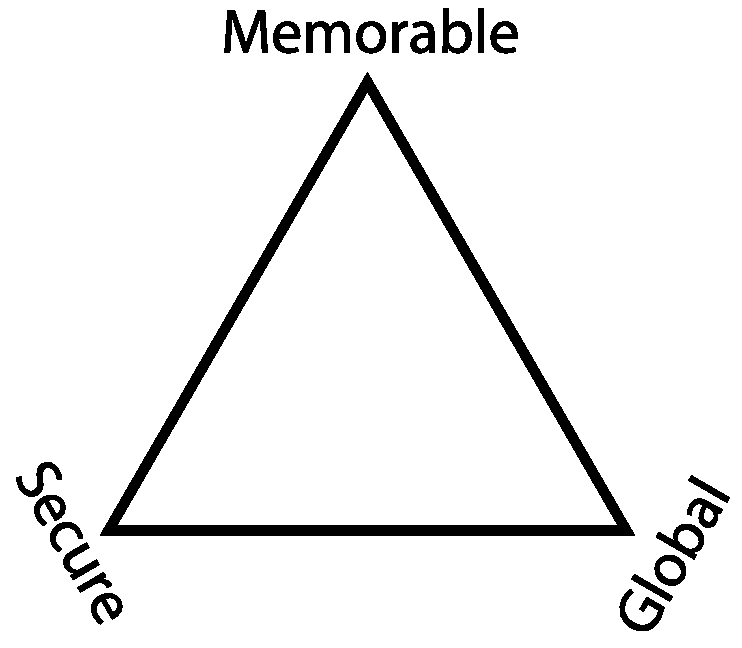
\includegraphics[width=\textwidth,height=0.2\paperheight,keepaspectratio
]{figures/Zooko_s_Triangle}
\caption{Zooko's Triangle, with the edges representing the achievable combinations of features \cite{Zooko:2001:Online}}
\label{fig:zooko}
\end{figure}

\section{Decentralization}
% Robert

Assuming that the system can utilize a DHT such as a cryptocurrency blockchain for storage of the public part of RSA key pairs, the issue of how to interface a web application with the blockchain in a way that allows for verification of identities without putting too much trust in the HTTP/cryptocurrency gateway also needs to be addressed. Additionally, as previously stated, the initial insertion of the key requires monetary resources, and is perhaps something that should be solved outside of Rymd.
While the public key can be stored in a DHT, private keys need to be stored securely on each client, preferably without giving client code any direct access to the raw keys. How the initial generation of keys are performed also needs consideration. Finally, a secure way to store the encryption keys for encrypted resources needs to be addressed. The question of how these resource-associated secret keys are distributed is deemed an implementation-specific question and will be out of scope for Rymd, but handled in Shuttle.

% "Centralized control – Distributed Data Architectures"
% http://highscalability.com/blog/2014/4/7/google-finds-centralized-control-distributed-data-architectu.html

\section{Encryption}
\label{sec:cryptography}

% Johannes

\section{Data Storage}
\label{sec:datastorage}
The storage of data was a crucial area to implement for a file sharing system. Since the data store was to be used by several parts of the application the demands for the module's interface had to be as general as possible, adhering to a standard CRUD\footnote{Create–Read–Update–Delete} interface, including methods for creating, fetching, updating and deleting records in the store.


\section{Modularity}

The system was designed from the ground up to use interchangeble parts. This was achieved by identifying key features and separating them into individual modules. These were then used and intertwined in a central hub.

Advantages

Dependency injection

\section{Testing}
\label{sec:testing}
Automatic unit tests have been implemented where possible. No integration or functional tests have been written for testing larger parts of the system, due to the fast iteration of the library's interface and constant change in the implementation. 
% TODO: more here?
